\documentclass[a4paper,11pt]{article}

% ====== PACKAGES ======
\usepackage[utf8]{inputenc}
\usepackage[margin=1cm]{geometry} % Margini ridotti per sfruttare lo spazio
\usepackage{tikz}
\usepackage{tabularx}
\usepackage{booktabs}
\usepackage{multicol}
\usepackage{fancyhdr}
\usepackage{array}
\usepackage{anyfontsize}

% ====== CARD MACROS ======
% Uniform 5.5x8.5 cm cards (slightly narrower to allow spacing)
\newcommand{\cardfront}[1]{%
	\begin{tikzpicture}
		\node[draw=black, thick, rounded corners=3mm, minimum width=5.5cm, minimum height=8.5cm, inner sep=0pt, fill=white] {
			\fontsize{100}{110}\sffamily\bfseries #1
		};
	\end{tikzpicture}%
}

\newcommand{\cardback}[1]{%
	\begin{tikzpicture}
		\node[draw=black, dashed, rounded corners=3mm, minimum width=5.5cm, minimum height=8.5cm, inner sep=0pt, fill=gray!5] {
			\fontsize{100}{110}\sffamily\bfseries #1
		};
	\end{tikzpicture}%
}

% ====== PLAYER SCORE CARD MACRO ======
\newcommand{\playerscorecard}{%
	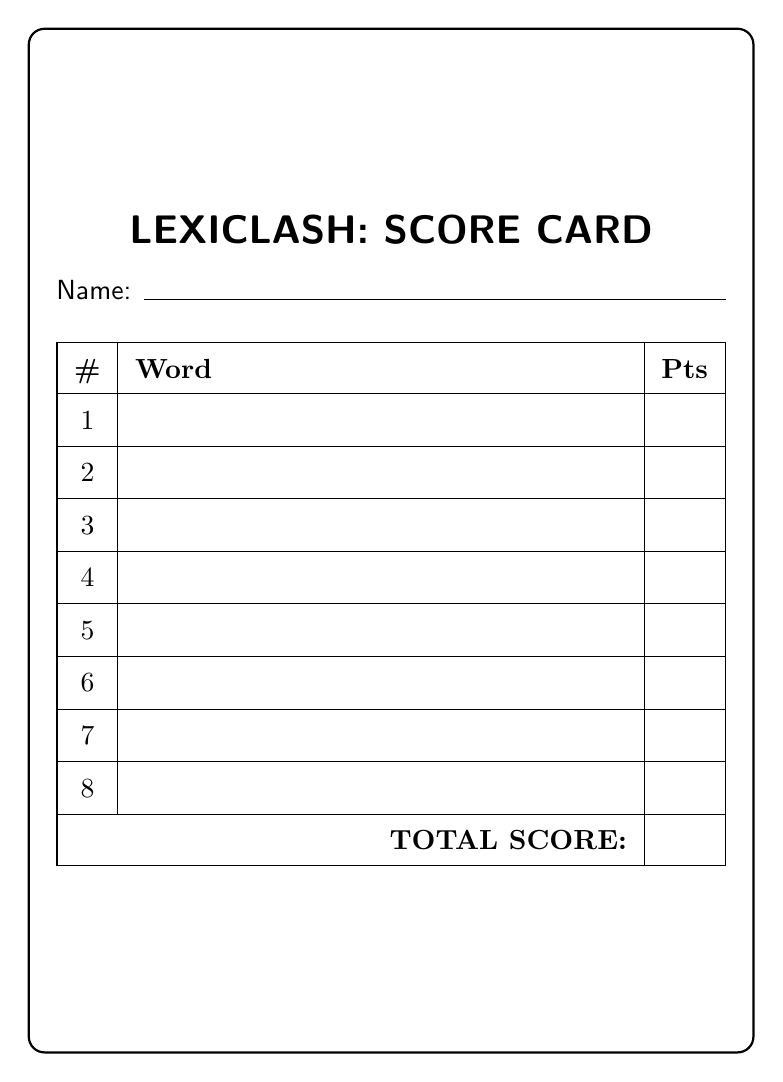
\begin{tikzpicture}
		\node[draw=black, thick, rounded corners=2mm, minimum width=9cm, minimum height=13cm, inner sep=10pt] {
			\begin{minipage}{8.5cm}
				\centering
				{\Large\sffamily\bfseries LEXICLASH: SCORE CARD} \\[0.3cm]
				\raggedright
				\textsf{Name:} \hrulefill \\[0.5cm]
				\centering
				\renewcommand{\arraystretch}{1.5}
				\begin{tabularx}{\linewidth}{|c|X|c|}
					\hline
					\textbf{\#} & \textbf{Word} & \textbf{Pts} \\
					\hline
					1 & & \\ \hline
					2 & & \\ \hline
					3 & & \\ \hline
					4 & & \\ \hline
					5 & & \\ \hline
					6 & & \\ \hline
					7 & & \\ \hline
					8 & & \\ \hline
					\multicolumn{2}{|r|}{\textbf{TOTAL SCORE:}} & \\ \hline
				\end{tabularx}
			\end{minipage}
		};
	\end{tikzpicture}%
}

% emptypage
\newcommand{\emptypage}{
	\clearpage
	\thispagestyle{empty}
	\hfill
	\clearpage
}

% Letters
\newcommand{\letters}{
	% --- PAGE 1: FRONT ---
	\begin{tabular}{c@{\hspace{0.8cm}}c@{\hspace{0.8cm}}c}
		\cardfront{A} & \cardfront{E} & \cardfront{I} \\[0.8cm]
		\cardfront{O} & \cardfront{U} & \cardfront{L} \\[0.8cm]
		\cardfront{N} & \cardfront{R} & \cardfront{T} \\
	\end{tabular}
	\newpage
	% --- PAGE 1: BACK ---
	\begin{tabular}{c@{\hspace{0.8cm}}c@{\hspace{0.8cm}}c}
		\cardback{1} & \cardback{1} & \cardback{1} \\[0.8cm]
		\cardback{1} & \cardback{1} & \cardback{1} \\[0.8cm]
		\cardback{1} & \cardback{1} & \cardback{1} \\
	\end{tabular}
	\newpage
	
	% --- PAGE 2: FRONT ---
	\begin{tabular}{c@{\hspace{0.8cm}}c@{\hspace{0.8cm}}c}
		\cardfront{D} & \cardfront{G} & \cardfront{B} \\[0.8cm]
		\cardfront{C} & \cardfront{M} & \cardfront{P} \\[0.8cm]
		\cardfront{F} & \cardfront{H} & \cardfront{V} \\
	\end{tabular}
	\newpage
	% --- PAGE 2: BACK ---
	\begin{tabular}{c@{\hspace{0.8cm}}c@{\hspace{0.8cm}}c}
		\cardback{3} & \cardback{2} & \cardback{2} \\[0.8cm] % Specchiato: B(3), G(2), D(2)
		\cardback{3} & \cardback{3} & \cardback{3} \\[0.8cm] % Specchiato: P(3), M(3), C(3)
		\cardback{4} & \cardback{4} & \cardback{4} \\        % Specchiato: V(4), H(4), F(4)
	\end{tabular}
	\newpage
	
	% --- PAGE 3: FRONT (Le 8 lettere mancanti + 1 'E' extra) ---
	\begin{tabular}{c@{\hspace{0.8cm}}c@{\hspace{0.8cm}}c}
		\cardfront{W} & \cardfront{Y} & \cardfront{K} \\[0.8cm]
		\cardfront{J} & \cardfront{X} & \cardfront{Q} \\[0.8cm]
		\cardfront{Z} & \cardfront{S} & \cardfront{E} \\
	\end{tabular}
	\newpage
	% --- PAGE 3: BACK ---
	\begin{tabular}{c@{\hspace{0.8cm}}c@{\hspace{0.8cm}}c}
		\cardback{5} & \cardback{4} & \cardback{4} \\[0.8cm] % Specchiato: K(5), Y(4), W(4)
		\cardback{10} & \cardback{8} & \cardback{8} \\[0.8cm] % Specchiato: Q(10), X(8), J(8)
		\cardback{1} & \cardback{1} & \cardback{10} \\       % Specchiato: E(1), S(1), Z(10)
	\end{tabular}
	\newpage
}

\setlength{\parindent}{0pt}

\begin{document}
	
	% ==========================================
	% SECTION 1: THE RULEBOOK
	% ==========================================
	\thispagestyle{empty}
	\begin{center}
		{\Huge \textsf{\textbf{LEXICLASH: STREET EDITION}}} \\[0.3cm]
		{\Large \textsf{The Offline Print \& Play Experience}} \\[1cm]
	\end{center}
	
	\section*{Game Overview}
	LexiClash is a fast-paced word-building game where players compete to find the most valuable word from a shared pool of letters.
	
	\section*{Components}
	\begin{itemize}
		\item \textbf{The Letter Deck:} A set of cards with a letter on the front and its point value on the back.
		\item \textbf{Score Sheets:} To track words, scores, and rounds.
		\item \textbf{Pens / Pencils:} Each player/team needs a pen to secretly write their words on their score sheet.
	\end{itemize}
	
	\section*{Setup}
	\begin{enumerate}
		\item Designate one person as the \textbf{Facilitator}. They will handle the deck and the Score Sheets.
		\item The \textbf{Facilitator} must separate the cards into \textbf{Vowels} and \textbf{Consonants} and shuffle the two decks.
		\item Distribute the Score Sheets to the players, having them write down their names or team names.
		\item Set the countdown timer.
		\item Determine the target score needed to win!
	\end{enumerate}
	
	\section*{How to Play (A Round)}
	The game is played over a series of rounds.
	\begin{enumerate}
		\item \textbf{Drawing Cards:} Proceeding counterclockwise, the active player tells the \textbf{Facilitator} how many \textbf{Vowels} and \textbf{Consonants} they want. The default number of cards drawn is 9, but the player can buy an extra slot by spending 10 points.
		\item \textbf{Starting the timer:} After all the requested letters have been dealt face up, the \textbf{Facilitator} starts the timer!   
		\item \textbf{Locking In:} Before the timer ends, players must secretly write their chosen word on their Score Sheet and put their pens down.
		\item \textbf{The Reveal \& Scoring:} Players reveal their words. The Facilitator checks if the words are valid and can be spelled using the available letters. 
		\item \textbf{Flipping for Points:} For each valid word, the Facilitator flips the used letter cards over to reveal their point values. Players sum their points to get their score for the round. \textit{Bonus: If a player manages to use all the available letters, their points for that round are doubled!} Record all points on the Score Sheets.
		\item \textbf{Cleanup:} The \textbf{Facilitator} discards the used cards. The turn then passes to the next player or team.
	\end{enumerate}
	
	\section*{Winning}
	The first player or team to reach the target score wins the game! 
	
	\newpage
	
	\emptypage
	
	% ==========================================
	% SECTION 2: PLAYER SCORE CARDS (4 per page)
	% ==========================================
	%\begin{center}
	%	{\Huge \textsf{\textbf{PLAYER SCORE CARDS}}} \\[0.5cm]
	%	\textit{Cut along the borders to distribute to players.}
	%\end{center}
	%\vspace{1cm}
	
	\centering
	\begin{tabular}{c@{\hspace{1cm}}c}
		\playerscorecard & \playerscorecard \\[1cm]
		\playerscorecard & \playerscorecard \\
	\end{tabular}
	
	\newpage
	\emptypage
	
	\centering
	\begin{tabular}{c@{\hspace{1cm}}c}
		\playerscorecard & \playerscorecard \\[1cm]
		\playerscorecard & \playerscorecard \\
	\end{tabular}
	
	\newpage
	\emptypage
	
	% ==========================================
	% SECTION 3: THE DECK
	% ==========================================
	% PRINTING: Flip on LONG EDGE.
	\centering
	
	\letters
	
	\letters
	
	\letters
	
\end{document}